\chapter{数据库设计}
\section{数据库环境说明}
%本系统的数据系统采用MySQL/PostgreSQL/Microsoft SQL Server数据库系统。

%其中xxx模块因为xxx而需要用到Hadoop架构。

本系统的数据系统采用MySQL数据库系统。

\section{数据库的命名规则及约定}
% 是否允许单词缩写,允许的单词缩写有哪些。
% %允许单词缩写
% %identity - ID
% %password - pw

% 表名是单数还是复数。关联表如何命名。字符数限制等。

% 字段是否带上前缀(如integer类型则加上i前缀等)。
%不带
本命名规则原则上遵循MySQL数据库官方推荐的命名规范。
\subsection{建表规范}
\begin{enumerate}
    \item 如无备注,则表中的第一个id字段一定是主键且为自动增长;
    \item 如无备注,则数值类型的字段请使用UNSIGNED属性;
    \item 如无备注,排序字段order\_id在程序中默认使用降序排列;
    \item 如无备注,所有字段都设置NOT NULL,并设置默认值;
    \item 如无备注,所有的布尔值字段,如is\_hot、is\_deleted,都必须设置一个默认值,并设为0;
    \item 所有的数字类型字段,都必须设置一个默认值,并设为0;
    \item 针对varchar类型字段的程序处理,请验证用户输入,不要超出其预设的长度;
    \item 建表时将数据字典中的字段中文名和属性备注写入数据表的备注中(“PK、自动增长”不用写);
    \item 如无说明,建表时一律采用innodb引擎;
\end{enumerate}

\subsection{表命名规范}
\begin{enumerate}
    \item 具备统一前缀,对相关功能的表应当使用相同前缀,如acl\_xxx,house\_xxx,ppc\_xxx;其中前缀通常为这个表的模块或依赖主实体对象的名字,通常来讲表名为:业务\_动作\_类型,或是业务\_类型;

    \item 表名使用英文小写单词,如果有多个单词则使用下划线隔开;

    \item 表名简介,使用常见单词,避免使用长单词和生僻词;

    \item 表引擎取决于实际应用场景及当前数据库中的已经存在的存储引擎;日志及报表类表应用myisam,与交易,审核,金额相关的表应用innodb引擎。总体来讲数据库默认innodb;

    \item 数据表必须有主键,且尽量均使用auto\_increment的id作为主键(与业务无关),和业务相关的要做为唯一索引;

    \item 默认使用utf8字符集(由于数据库定义使用了默认,数据表可以不再定义,但为保险起见,应都写上);
\end{enumerate}

\subsection{常用表名约定}
说明:表前缀用项目名称首字母缩写;所以表名都小写,单词之间用下划线分开,单词都用单数形式

\begin{enumerate}
    \item user – 用户
    \item category – 分类
    \item goods – 商品、产品等一切可交易网站的物品都用此命名
    \item good\_gallery – 物品的相册
    \item good\_cate – 物品的分类,除了单独作为表名,其他地方分类单词一律用缩写cate
    \item attr – 属性
    \item article – 文章、新闻、帮助中心等以文章形式出现的,一般都用此命名
    \item cart – 购物车
    \item feedback – 用户反馈
    \item order – 订单
    \item site\_nav – 包括页头和页尾导航
    \item site\_config – 系统配置表
    \item admin – 后台用户 【RBAC标准表】
    \item role – 后台用户角色【RBAC标准表】
    \item access – 后台操作权限,相当于action【RBAC标准表】
    \item role\_admin – 后台用户对应的角色【RBAC标准表】
    \item access\_role – 后台角色对应的权限【RBAC标准表】
\end{enumerate}

\subsection{字段命名规范}
\begin{enumerate}
    \item 数据库字段命名与表名命名类似:

    \item 使用小写英文单词,如果有多个单词使用下划线隔开;

    \item 使用简单单词,避免生僻词;

    \item 字段应当有注释,描述该字段的用途及可能存储的内容,如枚举值则应将该字段中使用的内容都定义出来;

    \item 是别的表的外键均使用xxx\_id的方式来表明;

    \item 表的主键一般都约定成为id,自增类型;

    \item 时间字段,除特殊情况一律采用int来记录unix\_timestamp;

    \item 网络IP字段,除特殊情况一律用bigint来记录inet\_aton值;

    \item 所有字段,均为非空,最好显示指定默认值;

    \item 有些驱动对tinyint支持不够好,通常建义按容量来选择字段;

    \item  text字段尽量少用,或是拆到冗余表中;
\end{enumerate}

\subsection{常用列名约定}
\begin{enumerate}
    \item 表名\_id – 通常用作外键命名
    \item cid – 特殊的编号,带有元数据,方便关联查询,你可以把它理解成类别(层次)编号。举个例子,产品在分类时,往往需要将其归类到子分类下,相应的字段中也一般只记录子分类的id,这时若需要知道该产品属于哪个主分类,就需要通过子分类信息再查询到主分类信息,这是比较麻烦的,cid字段就是要解决这个问题。一般的站点几十个分类肯定是够用了,所以这里假设某一主分类的cid为11,则子分类的cid从1101开始编号,处理时只需截取前两位数值便可知道该产品属于哪一个主分类了。
    \item add\_time – 添加时间、上架时间等
    \item last\_time – 最后操作时间,如登录、修改记录
    \item expire\_time – 过期时间
    \item name – 商品名称、商家名称等,不要跟title混用,title只用于文章标题、职称等
    \item price – 价格
    \item thumb – 只要是列表页面中的窗口图,一律用此命名
    \item image\_src – 相册中的图片地址一律用此命名,不要出现各种img,image,img\_url,thumb\_url等
\end{enumerate}

\section{逻辑设计}
%是否需要满足某一种范式。
逻辑设计需要满足BCNF范式。
\begin{figure}[h]
	\centering
	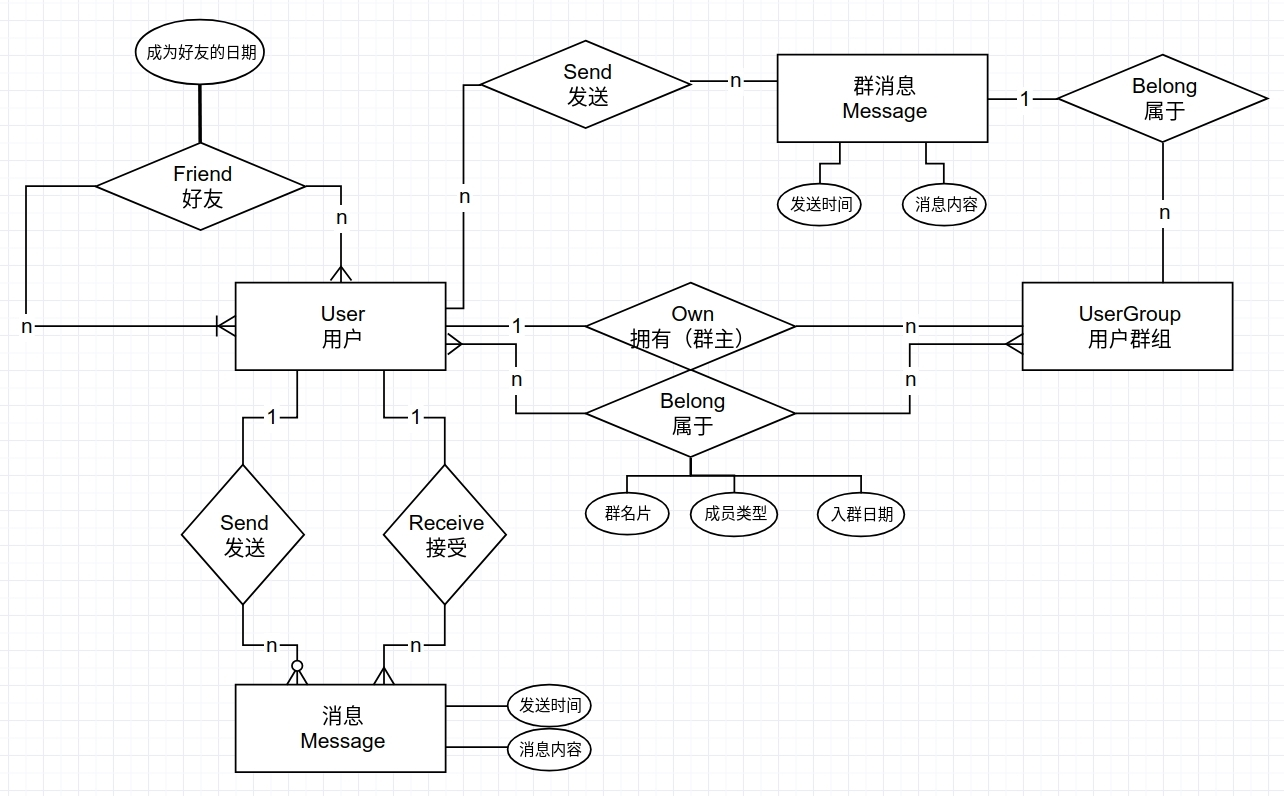
\includegraphics[width=15cm]{er_graph.jpg}
	\caption{ER图} \label{fig:er_graph}
\end{figure}
服务端数据库的E-R图如图-\ref{fig:er_graph}:。

\section{物理设计}
\subsection{数据库产品}
%用哪家数据库,是否分布式等。
使用MySQL 8.0。{\color{red} \sout{由于本产品可自主搭建与部署,且设计为小规模用户使用,故未考虑分布式存储需求。}\par}

\subsection{实体属性、类型、精度}
\subsubsection{客户数据表设计}

\begin{table}[htbp]
	\centering
	\caption{用户数据表Users设计} \label{tab:client-database}
	\begin{tabular}{|c|c|c|c|c|}
		\hline
		字段名       & 类型 & 大小 & 说明                 & 备注 \\
		\hline
		ID           & char & 64   & 用户的唯一标识符     & 主键 \\
		\hline
		pw           & char & 512  & 用户的登录密码hash值 & ·    \\
		\hline
		email        & char & 64   & 用户的注册邮箱       & 唯一 \\
		\hline
		lastlogin    & DateTime & 16   & 最近登录时间         & ·    \\
		\hline
		registertime & DateTime & 16   & 注册时间             & ·    \\
		\hline
		birthday     & Date & 16   & 生日                 & ·    \\
		\hline
		sex          & char & 4    & 性别                 & ·    \\
		\hline
		intro        & char & 512  & 个人说明             & ·    \\
		\hline
        avatar       & char & 512  & 头像url              & ·    \\
        \hline
        is\_active   & bool & 1    & 是否在线             & ·    \\
        \hline
        enable\_mobile\_notify & bool & 1 & 移动客户端是否启用消息通知 & · \\
        \hline
        enable\_desktop\_notify & bool & 1 & 桌面客户端是否启用消息通知 & · \\
        \hline
        enable\_sounds & bool & 1  & 是否静音             & ·    \\
        \hline
        default\_language & char & 20 & 默认显示语言       & ·    \\

    \end{tabular}
\end{table}
见表-\ref{tab:client-database}。

\subsubsection{好友数据表设计}
\begin{table}[htbp]
	\centering
	\caption{好友数据表Friends设计} \label{tab:friend-database}
	\begin{tabular}{|c|c|c|c|c|}
		\hline
		字段名 & 类型 & 大小 & 说明           & 备注                 \\
		\hline
		user1  & char & 64   & 用户1          & 外键,来自用户数据表 \\
		\hline
		user2  & char & 64   & 用户2          & 外键,来自用户数据表 \\
		\hline
		time   & Date & 16   & 成为好友的日期 & ·                    \\
		\hline
	\end{tabular}
\end{table}
见表-\ref{tab:friend-database}。

\subsubsection{消息数据表设计}
\begin{table}[htbp]
	\centering
	\caption{消息数据表Messages设计} \label{tab:message-database}
	\begin{tabular}{|c|c|c|c|c|}
		\hline
		字段名  & 类型 & 大小 & 说明             & 备注                 \\
		\hline
		ID      & number & 64   & 消息的唯一标识符 & 主键                 \\
		\hline
		time    & Date & 16   & 发送时间         & ·                    \\
		\hline
		content & char & 1000 & 消息内容         & ·                    \\
		\hline
		from    & char & 64   & 发送者           & 外键,来自用户数据表 \\
		\hline
		to      & char & 64   & 接收者           & 外键,来自用户数据表 \\
		\hline
	\end{tabular}
\end{table}
见表-\ref{tab:message-database}。

\subsubsection{群组消息数据表设计}
\begin{table}[htbp]
	\centering
	\caption{群组消息数据表Messages设计} \label{tab:groupmessage-database}
	\begin{tabular}{|c|c|c|c|c|}
		\hline
		字段名  & 类型 & 大小 & 说明             & 备注                 \\
		\hline
		ID      & number & 64   & 消息的唯一标识符 & 主键                 \\
		\hline
		time    & Date & 16   & 发送时间         & ·                    \\
		\hline
		content & char & 1000 & 消息内容         & ·                    \\
		\hline
		from    & char & 64   & 发送者           & 外键,来自用户数据表 \\
		\hline
		to      & char & 64   & 群组           & 外键,来自群组数据表 \\
		\hline
	\end{tabular}
\end{table}
见表-\ref{tab:groupmessage-database}。

\subsubsection{群组数据表设计}
\begin{table}[htbp]
	\centering
	\caption{群组数据表Groups设计} \label{tab:group-database}
	\begin{tabular}{|c|c|c|c|c|}
		\hline
		字段名     & 类型 & 大小 & 说明             & 备注                 \\
		\hline
		ID         & number & 64   & 群组的唯一标识符 & 主键                 \\
		\hline
		name       & char & 64   & 群名             & ·                    \\
		\hline
		intro      & char & 512  & 简介             & ·                    \\
		\hline
		createtime & Date & 16   & 创建日期         & ·                    \\
		\hline
		user       & char & 64   & 群主             & 外键,来自用户数据表 \\
		\hline
	\end{tabular}
\end{table}
见表-\ref{tab:group-database}。

\subsubsection{群组成员数据表设计}
\begin{table}[htbp]
	\centering
	\caption{群组成员数据表设计} \label{tab:usergroup-database}
	\begin{tabular}{|c|c|c|c|c|}
		\hline
		字段名     & 类型 & 大小 & 说明     & 备注                 \\
		\hline
		user       & char & 64   & 用户     & 外键,来自用户数据表 \\
		\hline
		group       & number & 64   & 群组     & 外键,来自群组数据表 \\
		\hline
		name       & char & 512  & 群名片   & ·                    \\
		\hline
		type       & char & 4    & 成员类型 & ·                    \\
		\hline
		createtime & Date & 16   & 入群日期 & ·                    \\
		\hline
	\end{tabular}
\end{table}
见表-\ref{tab:usergroup-database}。


\section{安全性设计}
%备份和容灾设计。
本产品的服务端主要面向有自己搭建即时通讯服务需求的个人用户和中小企业用户,
预期使用规模较小,所以没有特别的容灾设计,
数据备份工作依靠服务端维护人员自行开展。

\section{数据库管理与维护说明}
对于数据库的维护,随时对数据库中的信息加以调试和保存备份。同样需要个工作人员进行系统的分析和用户的反馈,对系统进行升级以及功能的完善。同时保证系统安全有序的运行。

{\color{red}
\section{一致性相关需求}
本系统在后期使用过程中可能会平均每秒都会面对上百万级的用户请求数。
}

{\color{red}
\section{检索速度相关需求}
本系统在后期使用过程中可能会平均会面对上亿级的用户规模。对于部分涉及到检索的功能需求而言,检索速度将成为功能操作的时间瓶颈。故检索速度在设计之初就需要仔细考虑。
\subsection{硬件要求}
在硬件上使用多个数据库专用服务器支持集群设计,
使用大内存服务来支持缓存技术。使用固态硬盘提高性能。


\subsection{读写分离}

\begin{figure}[h]
	\centering
	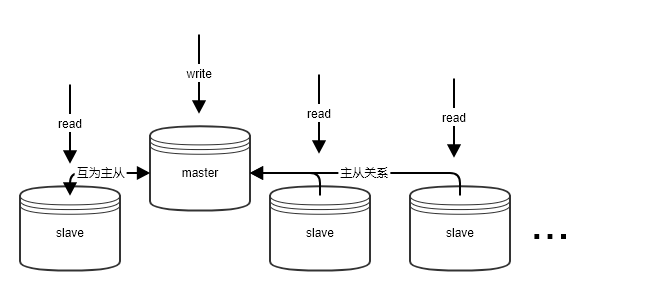
\includegraphics[width=13cm]{Read_Write_Splitting}
	\caption{读写分离} \label{fig:Read_Write_Splitting}
\end{figure}

见图-\ref{fig:Read_Write_Splitting}。
master 提供数据库写服务,slave 提供数据库读服务,两者直接通过 mysql 的 binlog 进行同步。
可通过横向扩展 slave 线性地增加读性能。
采用双机热备份。当 master 挂了,和 master 为主从关系的 slave 被停止访问,这时互为主从的slave负责读和写。
当 master 重新恢复后,slave 同步数据给 master,然后再次恢复最初读写状态。


\subsection{缓存}
相对于磁盘IO,内存的访问速度要快的多。使用内存数据库 redis 作为数据库缓存,加快数据库的访问速度。


\subsection{建立索引}
对于一些经常被查询的数据,需要建立索引以提高检索速度。
在本系统中,需要对用户表中的用户名建立索引,群组表中的群组名建立索引


\subsection{数据库拆分}
当表记录数达到千万甚至亿级别时,数据库表的访问效率下降明显,导致外层应用的访问效率非常差,访问时间急剧上升,用户体验下降。
对数据库表进行水平切分,降低单库数据容量,提升数据库性能


}